
%%%%%%%%%%%%%%%%%%%%%%%%%%%%%%%%%%%%%%%%%%%%%%%%%%%%%%%%
% LaTex Template for proposals within the              %
% DFG Research Unit Program                            %         
%Planet Formation Witnesses and Probes: Transition Discs
% August 2016                                            %                           
%                                                      %
%%%%%%%%%%%%%%%%%%%%%%%%%%%%%%%%%%%%%%%%%%%%%%%%%%%%%%%%
%
% 
%
% This template may be used to prepare proposals in latex.
%
%
% The project description, including publication list, should be no more than 20 pages
% in length. It should be self-explanatory and not require reviewers to read the 
% literature that is quoted or enclosed.

\documentclass[10pt,fleqn,twoside]{article}

%%%%%%%%%%
%% Packages (Kley)
\usepackage{journals}
\usepackage[breaklinks,unicode,colorlinks,linktocpage,pdftex,citecolor=black,linkcolor=black,urlcolor=blue,backref,pagebackref,bookmarks,bookmarksnumbered]{hyperref}
\newcommand{\beq}{\begin{equation}}
\newcommand{\eeq}{\end{equation}}
\newcommand{\sub}[1]{_{\rm #1}}
\newcommand{\PLUTO}{{\it PLUTO}}
\newcommand{\FARGO}{{\it FARGO}}
\newcommand{\PLATO}{{\it PLATO}}
\newcommand{\Gaia}{{\it Gaia}}
\newcommand{\BinAC}{{\it BinAC}}
%%  End Packages Kley

%%%%%%%%%%%%%%%%% GET THE STYLE STUFF %%%%%%%%%%%%%%%%%%%

%%%% USE ARIAL FONT %%%%%%%%%%%%%%%%%%%%%%%%%%%%%%%%%%%%%%%%%%%%%%%%%%%%%%
\usepackage{helvet}
\renewcommand\familydefault{phv}

%%%% INCLUDE NECESSARY PACKAGES %%%%%%%%%%%%%%%%%%%%%%%%%%%%%%%%%%%%%%%%%%
%\usepackage{babel}
\usepackage[UKenglish]{babel}
\usepackage{amsmath}
\usepackage{amssymb}
\usepackage{fancyhdr}
\usepackage{natbib}
\usepackage{ae,aecompl}
\usepackage{graphicx}
\usepackage{palatino}
\usepackage[T1]{fontenc}
\usepackage[right]{eurosym}
\usepackage{rotating}
\usepackage{epsf}
\usepackage{setspace}
\usepackage{xspace}
\usepackage{multicol}
\usepackage{siunitx}
%\usepackage{caption}

\usepackage{sfmath}

\usepackage[utf8]{inputenc}

% ========= hyperref & Colors & Links ===========
\usepackage[usenames,dvipsnames]{xcolor}
%\usepackage[breaklinks]{hyperref}
\usepackage{hyperref}
\addto\extrasUKenglish{%
\def\sectionautorefname{Section}%
\def\subsectionautorefname{Section}%
\def\subsubsectionautorefname{Section}%
\def\paragraphautorefname{Section}%
}
\usepackage[all]{hypcap} % fixes links to floats
\usepackage{aas_macros}  %
\setlength{\bibsep}{-0.5pt}

% ========= highlighting important parts of the proposal ===========
\definecolor{HighLight}{rgb}{0.9,0.3,0.0}
%\newenvironment{highlight}{\color{blue}\itshape}{\ignorespacesafterend}
%\newenvironment{highlight}{\color{RedOrange}\itshape}{\ignorespacesafterend}
%\newenvironment{highlight}{\color{RedOrange}\bfseries}{\ignorespacesafterend}
%\newenvironment{highlight}{\color{BrickRed}\bfseries\itshape}{\ignorespacesafterend}
%\newenvironment{highlight}{\color{BrickRed}\bfseries}{\ignorespacesafterend}
%\newenvironment{highlight}{\color{HighLight}\bfseries}{\ignorespacesafterend}
\newenvironment{highlight}{\color{HighLight}}{\ignorespacesafterend}
\newenvironment{missingenv}{\color{red}}{\ignorespacesafterend}

\definecolor{Emphasize}{rgb}{0.0,0.5,0.0}
\newenvironment{Emphasize}{\color{Emphasize}\itshape}{\ignorespacesafterend}


% strike through comments: to turn them off, uncomment the renewcommands below
\usepackage{soul}
\setstcolor{red}

% ========= Commands specially for the forschergruppe =========

\newcommand{\todo}[1]{\textcolor{red}{\bf #1}}
\newcommand\connect[1]{{\color{OliveGreen} #1}}

%%%% CAPTION LAYOUT %%%%%%%%%%%%%%%%%%%%%%%%%%%%%%%%%%%%%%%%%%%%%%%%%%%%%

\usepackage[font={small}]{caption}

%%%% PAGE LAYOUT %%%%%%%%%%%%%%%%%%%%%%%%%%%%%%%%%%%%%%%%%%%%%%%%%%%%%%%%%
\setlength{\textheight}{22cm}
\setlength{\topmargin}{-1.2cm}
\setlength{\textwidth}{15.6cm}
\setlength{\oddsidemargin}{0.0cm}
\setlength{\evensidemargin}{0.0cm}
\setlength{\mathindent}{1.5cm}
\setlength{\parindent}{0.0cm}
\setlength{\parskip}{0.08cm}

%%%% PAGE HEADER %%%%%%%%%%%%%%%%%%%%%%%%%%%%%%%%%%%%%%%%%%%%%%%%%%%%%%%%%%
\pagestyle{fancy}
\fancyhead[RE,RO]{}
\fancyfoot[RO]{\thepage}
\fancyfoot[LE]{\thepage}
\fancyfoot[CE,CO]{}

%%% FONTS FOR THE TITLE PAGE %%%%%%%%%%%%%%%%%%%%%%%%%%%%%%%%%%%%%%%%%%%%%%
\newfont{\tpfonta}{cmssbx10 scaled 1600}
\newfont{\tpfontb}{cmssbx10 scaled 3200}

%%%% COLOR DEFINITIONS %%%%%%%%%%%%%%%%%%%%%%%%%%%%%%%%%%%%
\definecolor{blue} {rgb} {0.25,0.25,0.75}

%%%% ADDITONAL EMPHASIS %%%%%%%%%%%%%%%%%%%%%%%%%%%%%%%%%%%
\newcommand{\cem}{\color{blue}}
\newcommand{\eem}{\sl\color{blue}}

%%%% BIBTEX PUNCTUATION %%%%%%%%%%%%%%%%%%%
\bibpunct{(}{)}{;}{a}{}{,} % to follow the A&A style

%%%% SET THE COLOR OF THE (SUB-) SECTION TITLES %%%%%%%%%%% 
\newcommand{\Tcol}{\color{blue}}

%%%% SET THE COLOR OF THE TITLE BOX BACKGROUND %%%%%%%%%%%%
\definecolor{Background}{rgb} {0.62,0.75,0.5}

%%%%%%%%%%%%%% REFERENCE SECTION NAME %%%%%%%%%%%%%%%%%%%%
\renewcommand\refname{\Tcol 9. Bibliography}

%%%%%%%%%%%%%% NICER PROJECT REFERENCES %%%%%%%%%%%%%%%%%%%

\newenvironment{literature}%
 {\begin{multicols}{2}\begin{scriptsize}\begin{list}{}{%
   \setlength{\topsep}{0em}%
   \setlength{\parskip}{0em}%
   \setlength{\parsep}{0em}%
   \setlength{\itemsep}{0em}%
   \setlength{\rightmargin}{0em}%
   \setlength{\leftmargin}{2em}%
   \setlength{\itemindent}{-2em}}}%
 {\end{list}\end{scriptsize}\end{multicols}}

%
% ...A compact itemize environment
%
\newenvironment{compactitemize}%
 {\begin{list}{$\bullet$}{%
   \setlength{\topsep}{0em}%
   \setlength{\parskip}{0em}%
   \setlength{\parsep}{0em}%
   \setlength{\itemsep}{0.0\baselineskip}%
   \setlength{\rightmargin}{0em}%
   \setlength{\leftmargin}{2.0em}%
   \setlength{\labelsep}{0.5em}%
   \setlength{\labelwidth}{1em}%
}}
 {\end{list}}

\newcounter{qcounter}
\newenvironment{compactenumerate}%
 {\begin{list}{\arabic{qcounter})~}{\usecounter{qcounter}%
   \setlength{\topsep}{0em}%
   \setlength{\parskip}{0em}%
   \setlength{\parsep}{0em}%
   \setlength{\itemsep}{0.0\baselineskip}%
   \setlength{\rightmargin}{0em}%
   \setlength{\leftmargin}{2.0em}%
   \setlength{\labelsep}{0.5em}%
   \setlength{\labelwidth}{1em}%
}}
 {\end{list}}

%%%% EXPLANATION FOR THE CONNECT COLOR %%%%%%%%%%% 
\newcommand{\footexplainconnect}{\footnote{The text highlighted in \connect{green} refers to the connection of this project to other projects of this Research Unit.}}
 
%%%%%%%%%%%%%%%%%% NICER REFERENCES %%%%%%%%%%%%%%%%%%%

%\usepackage[capitalise,nameinlink]{cleveref}
\newcommand{\cref}[1]{\autoref{#1}}

%%%%%%%%%%%%%%%%%% COLOR THE SECTION NUMBERS %%%%%%%%%%%%%%%%%

\makeatletter
\renewcommand\@seccntformat[1]{\color{blue} {\csname the#1\endcsname}\hspace{0.5em}}
\makeatother
\renewcommand\thesection{\arabic{section}.}
\renewcommand\thesubsection{\arabic{section}.\arabic{subsection}}

%%%%% color sections
\usepackage{sectsty}
\allsectionsfont{\color{blue}}


%%%% CHANGE THE APPEARANCE OF THE \PARAGRAPH COMMAND  %%%%%%%%%%%%%%%%%%%%%%%%%%%%%%%
\makeatletter
\renewcommand\paragraph{\@startsection{paragraph}{4}{\z@}%
            {-2.5ex\@plus -1ex \@minus -.25ex}%
            {1.25ex \@plus .25ex}%
            {\normalfont\normalsize\bfseries\Tcol}}
\makeatother
\setcounter{secnumdepth}{4}     % how many sectioning levels to assign numbers to
\setcounter{tocdepth}{4}        % how many sectioning levels to show in ToC

%%%%% set header

\renewcommand{\sectionmark}[1]{\markright{\color{black}#1}}

\newcommand{\caphighlight}[1]{{\bf #1}}



%%%%%%%%%%%%%%%%% DEFINE THE HEADER TEXT %%%%%%%%%%%%%%%%

\fancyhead[LE,LO]{\slshape
%%%%  Please edit
%
Wilhelm Kley: Transition disks and planetary systems (D1)}
%
%
%%%%%



\begin{document}


\newpage

%%%% PROJECT DESCRIPTION STARTS HERE %%%%%%%%%%%%%%%%%%%%%%%%%%%%%%%%%%%

\setcounter{page}{1}

\centerline{\huge\bf\Tcol
%
%
%
%
%%%%  Please edit
%
 Project D1:}
\vspace{1em}

\centerline{\LARGE\bf\Tcol Transition disks and planetary systems}

%
%%%%
%
%
%
%
\vskip1.0cm

%%%%  Please edit

\noindent{\bf Authors:}\\
\begin{tabular}{ll}
{\textsf{PI:}}               & W.~Kley (T\"ubingen)\\
{\textsf{Co-PI:}}             & C.P.~Dullemond (Heidelberg)\\
{\textsf{Collaborations:}}     & L.~Testi (ESO), E.~van Dishoeck (MPE), T.~Henning (MPIA)\\
\end{tabular}

%%%%  Please edit

\vspace{1em}
\noindent{\bf Requested positions: 1 Postdoc} \\

\vspace{1em}
\noindent{\bf Abstract:}\\
Transitional disks (TDs) presumably occur in the later phases of the evolution of
protostellar disks around young stars and show a depletion of flux from the inner, central parts of the disk.
One variety of such disks display a lack of radiation in the mid-infrared wavelength regime which is interpreted
as large inner holes in their dust distribution.
Nevertheless they show significant gas accretion signatures coming from the central inner region. 
It has been suggested that for these type of TDs this inner cavity might be
created by the presence of one or more planets that cleared out the inner disk region.
In this project we shall follow this line of thought and will perform multi-dimensional hydrodynamic studies
to clarify the dynamical impact of planets on TDs in order to prove (or disprove) the existence of planets in such disks.
The studies will include gas dynamics, dust particles, embedded planets, radiation transport
and irradiation from the central star.

\section{State of the art and preliminary work}
\renewcommand{\leftmark}{\sc State of the Art and preliminary work}
Observationally, transition disks are characterized by a lack of
flux in the few $\mu$-meter (near/mid IR) range as seen in the spectral energy distributions
(SEDs) of young stars. This flux deficit is typically associated with
'missing' dust having temperatures of 200-1000 K 
\citep{2002ApJ...568.1008C,2005ApJ...621..461D}
corresponding to the inner regions of accretion disks. Despite this lack of dust,
there are nevertheless still signatures of gas accretion in several systems with large inner (dust) holes
that are a few tens of AU wide. 

The observational properties of transitional disks and the modeling attempts up to date
have been reviewed recently by \citet{2016PASA...33....5O} and we mention here only the main aspects 
relevant to this project.
As described in the general introduction to this collaborative research proposal,
the origin of the inner disk clearing has been basically attributed to two different processes:
either photoevaporation from inside out through high energy radiation from the central young protostar
\citep[e.g.][]{1993Icar..106...92S,2006MNRAS.369..216A}, 
or by embedded massive planets that carve deep gaps into the disk \citep[e.g.,][]{2006ApJ...640.1110V}.
Now, as outlined in the introduction, TDs appear to come in two flavors, 
mm-faint disks with low mm-fluxes, small inner holes ($\lesssim 10$au), and low accretion rates
onto the stars ($\approx 10^{-10} - 10^{-9}$ M$_\odot$/yr)
and mm-bright-disks with large mm-fluxes, large holes ($\gtrsim 20$au), and high accretion rates
$\approx 10^{-8}$ M$_\odot$/yr \citep{2012MNRAS.426L..96O} to which we
refer here as  
Type I and Type II disks, respectively.

While photoevaporation is certainly at work in some systems (Type I TDs) it is believed that it can only
operate for systems with a sufficiently low mass accretion rate below $10^{-8} M_\odot/yr$
and is otherwise quenched by the accretion flow \citep{2012MNRAS.426L..96O}.
At the same time the persistence of gas accretion within the inner (dust) holes is taken as an additional
indication that other mechanisms should operate that create these gaps \citep{2014A&A...568A..18M}.
%  http://cdsads.u-strasbg.fr/abs/2014A%26A...568A..18M
The very likely mechanism for this second class of TDs is related to the growth of planets in the disks,
because young planets embedded in their nascent disks will not only
open a gap in the gas disk but they will create an even stronger
depletion of the dust near the planetary orbit \citep{2004A&A...425L...9P}.

Consequently, it has been suggested early on that the presence of a massive (Jupiter-sized) planet might be responsible for the
gap creation \citep{2006ApJ...640.1110V,2006MNRAS.373.1619R},
%, ApJ, 640, 1110; http://cdsads.u-strasbg.fr/abs/2006ApJ...640.1110V
%, MNRAS, 373,1619;  http://cdsads.u-strasbg.fr/abs/2006MNRAS.373.1619R
but at the same time it has been noticed that the gap created
by a single embedded planet is significantly narrower than
observations of transition disks suggest.
Given the problems with a single planet and the photoevaporation models, it has been proposed that the main observational
features can be created by the presence of a system of (three to four) massive planets.
Following this line of thought, \citet{2011ApJ...729...47Z}
% Zhu et al. (2011) , ApJ, 729, 47; http://cdsads.u-strasbg.fr/abs/2011ApJ...729...47Z
and \citet{2011ApJ...738..131D}
%  Dodson-Robinson \& Salyk (2011)
%, ApJ, 738, 131; http://cdsads.u-strasbg.fr/abs/2011ApJ...738..131D
performed numerical simulations and argue that transitional disks are in fact {\itshape Signposts of young multi-planet systems}.
In this scenario the embedded planets act as a 'barrier' for the gas flow through the disk allowing some
gas to enter the inner region, causing the observed accretional features near the star, while the dust
is filtered out at the pressure maximum just beyond the outer edge of the gap and cannot enter the inner disk regions.
Following this line of thought theoretical models with embedded planets and dust in disks
have been constructed to match the observed spectral energy distributions in the sub-millimeter
\citep{2013A&A...560A.111D,2015A&A...573A...9P}. However, even though the disk is modeled via
two-dimensional (2D) hydrodynamical simulations in this case the dust motion is not 
self-consistent and based on the azimuthally averaged
disk models using a 1D dust evolution model of \citet{2010A&A...513A..79B}.

New ALMA observations in special wavelength bands focusing on CO-vibrational lines have allowed
to determine the gas content in the inner disk region in more detail. These results show that 
the inner disk gas depleted by factors of about $10^{2}$ \citep{2015A&A...579A.106V} or even to a factor
of $10^{4}$ with gas holes about a factor 2-3 smaller than the dust gaps \citep{2016A&A...585A..58V}
which is taken as another example of massive planets in disks \citep{2016Natur.530..169H}.
The conclusion that all or the majority of Type II TDs are shaped by massive planets has been
questioned recently by \citet{2016ApJ...825...77D} who argue that
there may not be enough giant planets to explain all observed Type 2 TDs, see also \citet{2008PASP..120..531C}
for the occurrence rate of massive planets at larger separations.
The solution to this problem is either that current numerical 
models of planet-disk interactions are too inefficient at gap opening compared to Nature, 
or that Type II TDs are intrinsically rare objects, rather than common and sort-lived objects, 
as is probably the case for their Type I counterparts. Considering that the arguments
of \citet{2016ApJ...825...77D} are based on analytical approximations on gap widths and sizes that
are based on isothermal models and do not consider any dust motion it may well be that the theoretical models
have not reached the degree of sophistication necessary to produce reliable results.
%% Until this question is answered the role of Type II TDs as “Signposts of young multiplanet systems” remains uncertain.

As pointed out above,  
despite this strong belief that planets play an important role in shaping transition disks, there
is still a lack of theoretical modeling to be able to make detailed comparison with observations.
The most advanced simulations are those of \citet{2011ApJ...729...47Z} who model a system of up to 4 massive planets embedded
in a 2D flat disk. Their studies suggest that only the presence of several planets will result in a
strong depletion of the gas in the inner disk. However, there are several short-comings. The simulations treat the disk in the
isothermal approximation, they are only 2D and neglect the vertical structure, and no accretion luminosity of the
planets was considered. Despite these limitations the most important constraints may be the omission of
dust particles in the simulations, which is important as it is the dust emission that is actually observed
in many cases.

In any event, as mentioned in the recent review by \citep{2016PASA...33....5O}: 
{\it if we understand the specific planet-disk signature, then we may be able to
use the observations of transition disks to observationally probe planet formation}.
In this project we aim exactly at this twofold goal: We will construct new self-consistent models 
for Type II TDs that contain a system of embedded planets that will allow us to determine
the role that planets play in shaping TDs in general, and obtain at the same time a deeper understanding of the planet
formation process.
Given that many of the above issues, as well as our modeling techniques, 
may also apply to the newly emerging class of ``Multi-Ringed Disks'' (such as HL Tau,
TW Hydra, HD 163296, BP Piscium, etc., see Introduction text of this Research
Unit), we will also include these objects in our scope.

To this purpose we will perform a series of time-dependent, multidimensional hydrodynamical 
simulations to study in detail the impact of a planetary system on the ambient disk. 
In these new studies we will go beyond the isothermal approach used
by most of the studies and will add radiative transport, including irradiation from the central star.
Secondly, the motion of embedded dust particles will be followed simultaneously with the gas
which allows to study in detail the gas motion and dust filtration process at the gap's outer edge as a function
of particle size. Thirdly, we will perform simulations in full 3D that allows us to study the gas overflow
across the planets in detail and makes the stellar irradiation more realistic. 
The results of the simulations will be used to calculate emission properties to be compared to the observations.

\subsection{Preliminary work}
The PI of this project has ample experience in modeling accretion disks with embedded planets, starting from single
embedded planets to a system of planets evolving into a resonant configuration. Initially two-dimensional (2D) studies
in the isothermal approximation were performed and later full 3D studies including full radiative transfer. 
A summary of the topic of planet-disk interaction with references to several works of the PI is given in a review
article in Annual Rev. of Astronomy \& Astrophysics by \citet{2012ARA&A..50..211K}.
The evolution of two massive planets embedded in a disk has been studied in \citet{2004A&A...414..735K} where
we were interested in the resonant capture process. In \citet{2006A&A...447..369K} we
studied the impact of circular embedded planets on an outer disk, and in
\citet{2009A&A...506..971K} we studied the planet-disk interaction in full 3D radiative disks. 
In the past years a study on the physics of transitional disk 
with one embedded massive planet has been conducted \citet{2013A&A...560A..40M},
and recently hydrodynamical simulations with embedded dust particles have 
been performed \citet{2015A&A...584A.110P,2016A&A...594A..57S}. 
Here, we list some of our recent work relevant to this project.

\subsubsection{On the accretion flow in Transitional Disks}
In \citet{2013A&A...560A..40M} two-dimensional hydrodynamical simulations using the grid-based code 
FARGO for disks with a single embedded planet were performed. 
In addition to the standard isothermal models we constructed models that include 
viscous heating,  radiative cooling from the disk surfaces, 
radiative diffusion in the disk midplane and stellar irradiation in the energy equation in order
to have more realistic models and estimate the importance of the disks thermodynamics on the flow.
The mass flow rate into the gap region depends, for given disk thermodynamics, non-monotonically
on the mass of the planet. Generally, more massive planets open wider and deeper gaps
which would tend to reduce the mass accretion into the inner cavity. However, for larger mass planets
the outer disk becomes eccentric \citep{2006A&A...447..369K} and the mass flow rate is enhanced over the low mass cases.
As a result, for the isothermal disks the mass flow into the inner gap is always comparable to the expected mass flow of
unperturbed disks $\dot{M}_\mathrm{d}$, while for radiative disks the mass flow is very small for
low mass planets ($\leq 4\,M_\mathrm{jup}$) and about 50\,\% of $\dot{M}_\mathrm{d}$ for larger planet masses.
The radial surface density distribution and the mass accretion rate into the inner disk cavity is shown
in Fig.~\ref{fig:ecc-mdot-time} for the $4 \,M_\mathrm{jup}$ planet located at 5.2au for different treatments of the disk
thermodynamics. As shown in the upper panel, the isothermal model shows by far the highest gas density
in the inner disk region, while the radiative models fall well below it. Including stellar irradiation
brings the models somewhat in between the purely isothermal and radiative case.
This gas density distribution is reflected in the mass accretion rate onto the star displayed in the bottom
panel of Fig.~\ref{fig:ecc-mdot-time}. 
In addition, for the radiative disks the critical planet mass for the disk to become eccentric is much larger
than in the purely isothermal case.
In \citet{2013A&A...560A..40M} we simulated only single embedded planets on fixed circular orbits
but we could show that massive embedded planets can reduce the mass flow across the gap considerably,
and that the disk thermodynamics plays indeed a decisive role in determining the gas fraction entering the inner hole.

\begin{figure}[t]
\centerline{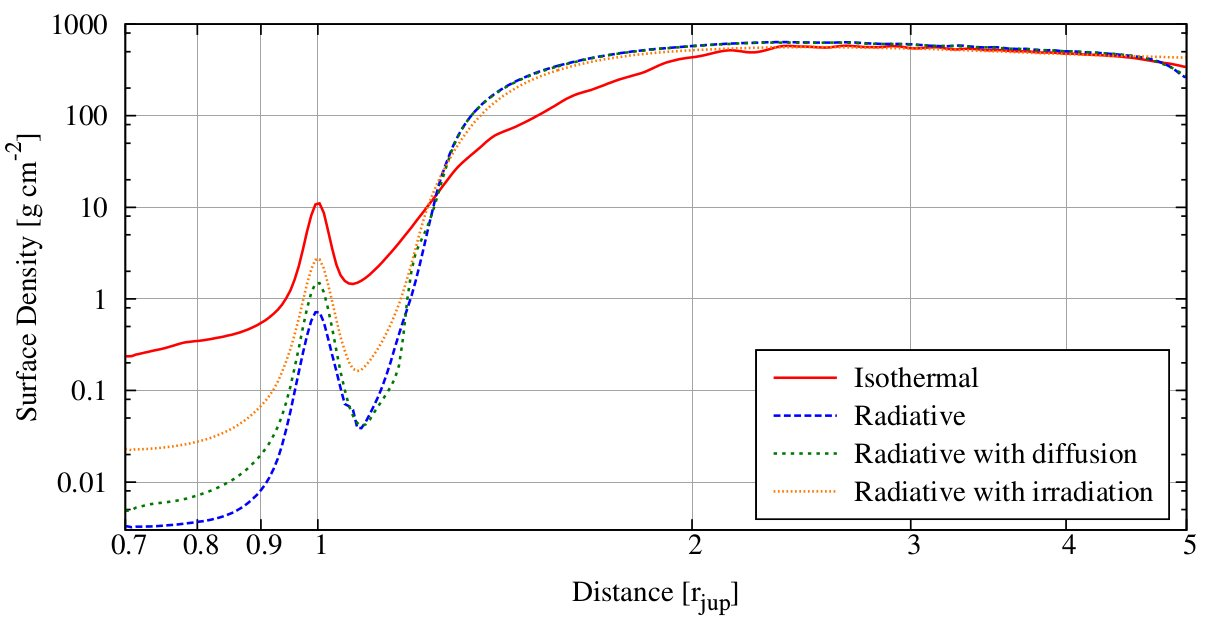
\includegraphics[width=0.75\textwidth]{pics/mueller-kley-2013-fig29.jpg}}
\centerline{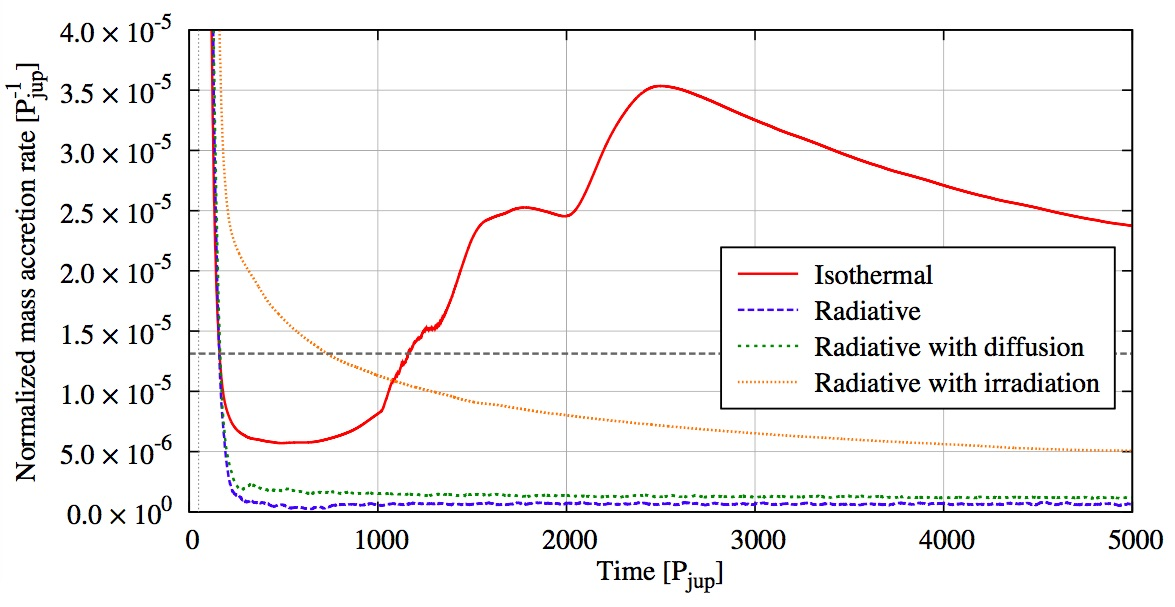
\includegraphics[width=0.77\textwidth]{pics/mdot-time-4MJup.jpg}}
\caption{\label{fig:ecc-mdot-time} Radial density distribution (\caphighlight{top
    panel}) and time evolution of the mass accretion rate (\caphighlight{bottom
    panel}) into the inner hole of the disk for a $4 M_{Jup}$ planet located
  at 5.2au in a transitional disk.  Shown are curves for different
  thermodynamic treatments of the disk physics.  Taken from:
  \citet{2013A&A...560A..40M}}
\end{figure}
%
\subsubsection{On the dust distribution in the disk around HL Tau}
%
Upon publication of the spectacular image of the ``Multi-Ringed Disk''
system in the HL~Tau disk by the ALMA Partnership
\citep{2015ApJ...808L...3A}, we
performed hydrodynamical simulations of the disk around HL~Tau with embedded planets and dust particles \citep{2015A&A...584A.110P}.
There, we followed the evolution of a population of dust particles treated as Lagrangian particles simultaneously with
the hydrodynamics, 
in two-dimensional locally isothermal disks where two equal-mass planets are present. 
The planets were kept in fixed orbits and they did not accrete mass. 
We found that the outer planet plays a major role in removing the dust particles in the co-orbital region of the 
inner planet and in forming a particle ring which has a steeper density gradient 
close to the gap edge with respect to the single-planet scenario, which promotes the development of vortices. 
The ring and gap width depend strongly on the planetary mass and particle stopping times of the particles,
i.e.\ how well they couple to the gas motion.
For the more massive cores the ring clumps into few points that are able to collect a high mass fraction.
In summary we found that the features observed in the HL Tau system can be explained
through the presence of two massive cores that shape the dust disk where the inner planet
has a mass of the order of $0.07 M_{Jup}$ and the outer one of the order of $0.35 M_{Jup}$. 
These values can be significantly lower if the disk mass turns out to be less than previously estimated. 
By decreasing the disk mass by a factor of 10, we obtain similar gap widths for planets with
a mass of $10 M_{Earth}$ and $20 M_{Earth}$ for the inner and outer planets, respectively. 
Although the particle gaps are prominent, the expected gaseous gaps are barely visible.
The final distribution of dust particles of different sizes is shown in Fig.~\ref{fig:particles},
clearly the gap width depends on the size or better the dimensionless stopping time of the embedded particles,
see eq.~(\ref{eq:tau-stop}) below.
For very small particles that couple well to the gas (top left panel) there is no strong gap visible
while for larger, not so well coupled particles a strong gap will be opened in the dust distribution.
Obviously this filtering effect will play a major role in determining the dust distribution in transitional disks as well.

\begin{figure}[t]
\centerline{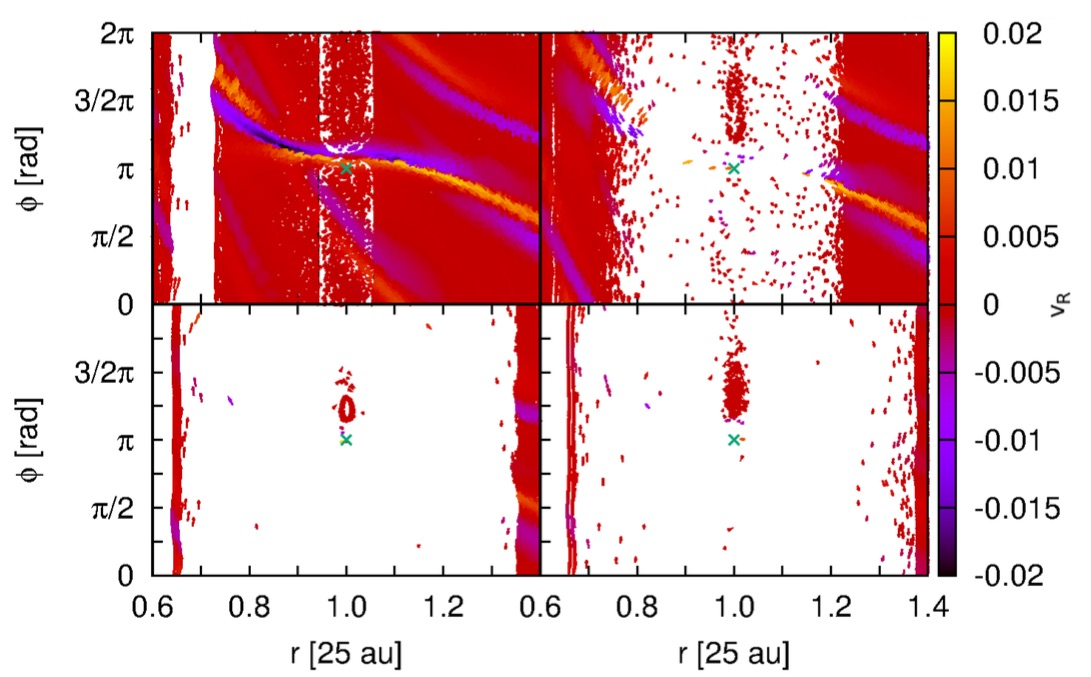
\includegraphics[width=0.75\textwidth]{pics/particles.jpg}}
\caption{\label{fig:particles} Particle distribution near the inner low mass
  planetary core location for mm- (\caphighlight{top left}), cm-
  (\caphighlight{top right}), dm- (\caphighlight{bottom left}), and m-sized
  (\caphighlight{bottom right}) particles at the end of the simulation.  The
  velocity vectors of the particles with respect to the planet are shown and
  the colour scale shows the relative radial velocity.  Taken from:
  \citet{2015A&A...584A.110P}}
\end{figure}

\subsubsection{Circumbinary disks and GPU-computing}
In a closely related project we studied the evolution of disks around a central
binary star (circumbinary disks, CBs) and followed the migration process of embedded planets
\citep{2014A&A...564A..72K,2015A&A...581A..20K}. This work is conceptually similar to the  
transitional disk case in that multiple objects (here two stars - in the TD case a few planets) are surrounded by an
outer disk which which is truncated due to the torques acting by the embedded bodies.
In both cases there is nevertheless a transfer of mass into the inner central region.
The CB-disk simulations were performed for 2D flat-disk configurations using the binary parameter of
the Kepler-38 and Kepler-34 system. In addition to locally isothermal runs we included
in some models viscous heating, and radiative cooling \citep{2008A&A...487L...9K}. 

To run such CB-disk and TD models as mentioned above \citep{2013A&A...560A..40M}
takes typically several 1000 dynamical timescales (e.g.\ orbit of the binary/planets) to bring the system
into quasi-equilibrium. For standard codes, even using the FARGO-algorithm, this requires considerable
computer time, see also the comments in \citet{2011ApJ...729...47Z}. Hence, within the
framework of a Diploma/PhD-Thesis, we have recently
developed a completely new implementation of the PLUTO-code to run on Graphics Processor Units (GPUs).
Presently, full 3D viscous hydrodynamics is included and for 2D disks we have implemented
radiative effects as well. In a first application we studied the dynamical friction process
\citep{2016A&A...589A..10T} and will submit a new paper on the dynamics of circumbinary disks shortly.
The CPU time used by this new code is shown in Fig.~\ref{fig:cpu} for a standard test-problem.
As can be inferred from the plot, the new GPU-code runs on one GPU card in our new cluster (see Sect.~\ref{sec:computers})
as fast as the pure MPI-version on about 60 cores.
In this project we plan to use this code in addition to the publicly available versions of the FARGO and PLUTO code.

\begin{figure}[t]
\centerline{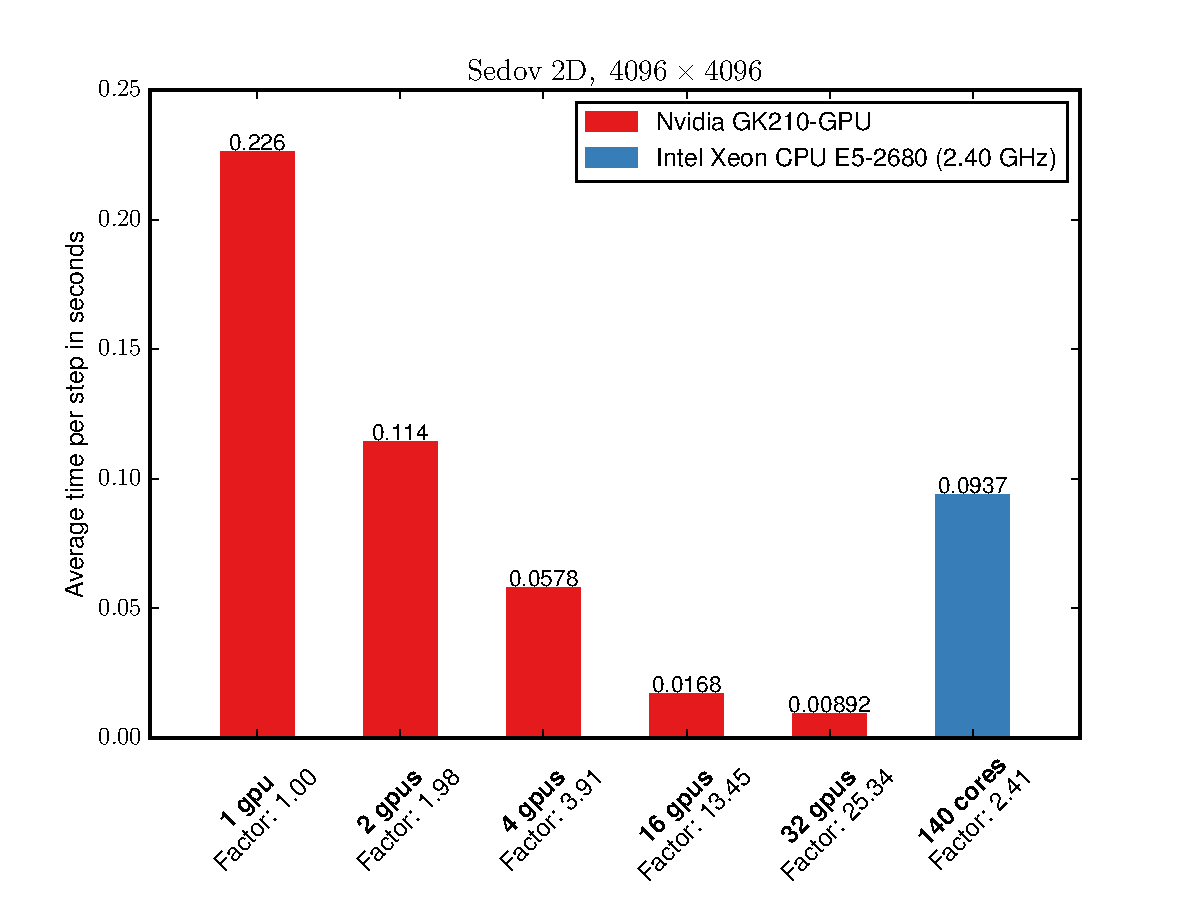
\includegraphics[width=0.75\textwidth]{pics/sedov2d_scaling.pdf}}
\caption{\label{fig:cpu} Computational time used for simulations using our new GPU-PLUTO code
on the 2D Sedov testproblem using $4096 \times 4096$ gridcells.
In red the values for the GPU-runs are displayed where multiple GPUs are connected via
MPI. Each node of the system has 4 GPUs, so the results for 16 and 32 GPUs includes MPI communication
between different nodes. The blue column refers to an MPI simulation on 5 nodes with 28 cores each.
} 
\end{figure}
%
\subsection{Project-related publications}

% Please list your own publications related to the proposed project, 
% adhering to the rules of the DFG guidelines 1.91. In brief, please note: 
% - Up to 10 publications
% - The work must be published or accepted.
% - Publications on astro-ph (arXive, SPIRES or articles with a DOI) count as published. 
% - Any work that is only in the status ``accepted'' MUST be attached to the proposal
%    together with the acceptance letter.
% - All publications in this section CAN be attached to the proposal. Please limit these
%    attachments to a minimum and please note that the reviewers may not read the attachments -
%    the proposal has to speak for itself.
% - The number of allowed publications refers to the sum of the publications listed
%    in ``1.1.1 Articles published or officially accepted by publication outlets...'' and 
%    in ``1.1.2 Other publications''. Publications which only exist on public repositories 
%    belong into the category ``Other Publications''.


%\subsubsection{
%A chronological list of selected relevant articles published or officially accepted by 
%publication outlets with scientific quality assurance.

\begin{literature}
\item {\bf Kley, W.}, \& Dirksen, G., {\em Disk eccentricity and embedded
    planets}, 2006, A\&A, 447, 369. In this paper we
  demonstrate how a massive planetary companion can make an outer disk eccentric. The applied
  methods and results are relevant at least for Task 1 of the project.
\item
 {\bf Kley}, W. \& {Crida}, A. (2008) \, {\it Migration of protoplanets in radiative disks},
   Astronomy \& Astrophysics, 487, 9.
  In this paper we present a detailed study of the importance of an improved thermodynamical
  treatment on the migration problem. The presented methods are directly relevant to the
  first Task of the project that deals with 2D disks including radiative transport and cooling.
\item {Gorti}, U., {\bf Dullemond}, C.~P. \& {Hollenbach}, D. (2009) \,
  {\it Time Evolution of Viscous Circumstellar Disks due to Photoevaporation by Far-Ultraviolet, 
   Extreme-Ultraviolet, and X-ray Radiation from the Central Star},
  Astrophysical Journal, 705, 1237.
  In this paper we describe a method on how to evolve viscous disks with photoevaporation
  due to high energy radiation. This porcess is important to clear out in inner regions particularly
  for type I TDs but may play a role for type II disks as well.
\item
  {\bf Kley}, W., {Bitsch}, B. \& {Klahr}, H. (2009) \,
  {\it Planet migration in three-dimensional radiative disks},
  Astronomy \& Astrophysics, 506, 971. 
  In this paper we study the interaction of an embedded planet with the disk in full 3D including radiative
  transport. This paper is relevant as demonstrate the importance of radiative transport on 
  planet disk interaction and we introduce here the treatment of radiative transport and the Fargo-algorithm
  in 3D hydrodynamics.  
\item
  {Kolb}, S.~M.; {Stute}, M.; {\bf Kley}, W. \& {Mignone}, A., 
  {\it Radiation hydrodynamics integrated in the PLUTO code},
   Astronomy \& Astrophysics, 559, A80. In this paper we describe the implementation of a new
   full 3D radiation module to the PLUTO-code using flux-limited diffusion including irradiation
   from the central star via ray-tracing. The new modules have been made available via webserver to
   the computational astrophysics community and are relevant for this project in particular Task 3.
\item
  {M{\"u}ller}, T.~W.~A. \& {\bf Kley}, W. (2013) {\it Modelling accretion in transitional disks}
   Astronomy \& Astrophysics, 572, A61.
  This paper shows our experience with modeling the dynamics of transition disks. In this paper
  the gas flow through the planet-induced gap is studied using various treatments of the disks thermodynamics.
  This is very relevant for the type 2 TDs which usually still have substantial accretion
  onto the star and have inner disks.
\item
 {Ataiee}, S., {Pinilla}, P., {Zsom}, A., {\bf Dullemond}, C.P., {Dominik}, C. \& {Ghanbari}, J. (2013)
   {\it Asymmetric transition disks: Vorticity or eccentricity?},
   Astronomy \& Astrophysics, 553, L3.
   This paper shows our work on how a
  massive planet can make the disk asymmetric (lopsided) in two independent
  ways: by making the disk eccentric or by creating a vortex. We show how to
  distinguish observationally between these two scenarios. It is 
  relevant with respect to the consideration of dust and hydrodynamics and is an example
  of how we make a link between modeling and observations.
\item
  {Picogna}, G. \& {\bf Kley}, W. (2015) \,
  {\it How do giant planetary cores shape the dust disk?. HL Tauri system},
  Astronomy \& Astrophysics, 584, A110. In this paper we present 2D disk simulations that simultanously
  evolve the disk, embedded planets and dust particles. It shows very clearly the different behaviour of gas
  and dust and the importance of incorporating both at the same time.
\item
  {\bf Kley}, W. \& {Haghighipour}, N. (2014) \,
  {\it Modeling circumbinary planets: The case of Kepler-38},
  Astronomy \& Astrophysics, 564, 72. The dynamical evolution of circumbinary disks with embedded planets 
  is calculated. We show that a migrating planet can naturally be stopped at the inner disk gap 
  close to the observed position. The paper is relevant as the overall dynamics of the system 
  (i.e. several bodies interacting with a disk) is similar to the problems to be treated here.
\item
  {Stoll}, M.H.R. \& {\bf Kley}, W. (2016) \,
  {\it Particle dynamics in discs with turbulence generated by the vertical shear instability},
  Astronomy \& Astrophysics, 594, A57. In this paper we describe the evolution of dust and gas for 3D
  accretion disks. The methodology applied here is important for the Task 3 of this project.
\end{literature}

%% \subsubsection{Other publications}
%%  [Text]

% \subsubsection{Patents}
% 
% \paragraph{Pending}
% 
% [Text]
% 
% \paragraph{Issued}
% 
% [Text]

\section{Objectives and work programme}
\renewcommand{\leftmark}{\sc Objectives and work programme}


\subsection{Anticipated total duration of the project}

3 years.

\subsection{Objectives}

The ultimate goal of this project is to investigate whether Type 2 TDs 
and/or Multi-Ringed Disks are signposts of (multiple) planet formation: 
i.e.\ can the observed features of these disks
be explained by an ensemble of embedded planets and what can we learn in this case about the nature
of the planets?
Earlier models have tried to explain TD holes with multi-planet systems, but their
conclusions are inconclusive due to missing essential physics, such as dust dynamics, radiative cooling and
full 3D flow.
In this project we plan to bring the modeling of Type II TDs and Multi-Ringed Disks 
that contain a system of embedded planets to a new level of realism
that allows robust predictions.
To this purpose we will perform a series of time-dependent, multidimensional hydrodynamical simulations to study in detail the impact of
a planetary system on the ambient disk. The new studies will first include realistic thermodynamics of the gas by adding radiative transport
and including irradiation from the central star. Secondly, the motion of embedded dust particles will be followed
which allows to study the gas dynamics and dust filtration process at the gap's outer edge.
Thirdly, we will perform simulations in full 3D that allows us to study the gas overflow
across the planets in detail and makes the stellar irradiation more realistic.
\connect{The results of the simulations will be used to calculate
  emission properties to be compared to the observations in
  collaboration with the A1 (PI Testi) team. A selection of the
  developed models will also be used by subprojects B1
  (photoevaporation PI Ercolano), B2 (chemistry PI Caselli \&
  Ercolano), C1 (PI Birnstiel \& Dullemond) and C2 (PI Ercolano).The
  models will be used to investigate the effects of planet-gaps in the
disk on photoevaporation (B1), search for chemical signature of
planet-induced gaps (B2), explore the effects of these gaps on dust
traps (C1) and on the final dust entrainment in the wind (C2)\footexplainconnect}.


\subsection{Work programme including proposed research methods}

%
The hydrodynamical simulations will make use of the FARGO- and {PLUTO}-codes.
Using the spatial distribution of the dust and gas we will use the radiative transport
code RADMC-3D for making observational predictions from our models.
The project will contain the following steps:

\begin{compactenumerate}
 \item {\it 2D hydrodynamical simulations of protoplanetary disks with multiple embedded planets} \\ 
To connect to existing multi-planet simulations of \citet{2011ApJ...729...47Z} 
   and our own \citep{2013A&A...560A..40M}
%% http://cdsads.u-strasbg.fr/abs/2013A%26A...560A..40M
   the first hydrodynamical models will be performed for flat 2D locally isothermal disks that
   contain several planets. In a parameter study the planetary masses will be varied systematically,
   and the resulting equilibrium density configurations will be analysed. The 2D isothermal models will
   be extended by including viscous heating, radiative cooling and transport based on \citet{2008A&A...487L...9K} and \citet{2012A&A...539A..18M}. 
%%   M\"uller \& Kley (2012).
%%  http://cdsads.u-strasbg.fr/abs/2012A%26A...539A..18M
  For these models first emission maps will be calculated using the RADMC-3D code \citep{2012ascl.soft02015D}.
\item {\it Dust evolution in 2D dimensional disk simulations with embedded protoplanets} \\
   Dust particles will then be added to these models whose motion is determined by the frictional forces between
   gas and particles, that depends on the particle size and the gas density of the disk. 
   In parameter studies the disk mass, the planet mass and the particle radii will be varied in order to
   determine the dust depletion factor within the central cavity relative to the gas accretion rate 
   as a function of particle size and planet masses. Additionally we will determine the accumulation point of the dust
   in the outer remaining disk and check for possible asymmetries.
   For this work we shall extend the methods developed in \citet{2015A&A...584A.110P}.
%%  Picogna \& Kley (2016).
%%  Picogna et al. 2016: http://cdsads.u-strasbg.fr/abs/2015A%26A...584A.110P
\item {\it Full three dimensional disk simulations with embedded protoplanets} \\
   From the 2D-runs the most promising parameter sets will be selected to perform full 3D time dependent
   hydrodynamical simulations using the {PLUTO}-code. These simulations will yield new results of the
   mass overflow across the planetary obits and allow for small inclinations of the planets.
   Using the resulting gas and dust spatial density distribution
   the RADMC-3D code will be applied for making observational predictions from our models.
   This can be used for both, continuum and line emission.
%% \item In the last part we will make the models more realistic and use an improved equation of state
%%     and internal (viscosity) as well as external (stellar irradiation) heat sources in the simulations.
%%     Accretional heating from the mass accretion of planet will be taken into account as well.
\end{compactenumerate}


\subsubsection{Tools for the proposed project}
\label{subsec:tools}
As the projects includes complex numerical hydrodynamical simulations we plan to
perform simulations with different numerical tools (codes) in order to crosscheck
our results. Experience has shown that the usage of different codes on the same
physical problem in parallel allows the elimination of numerical issues and improves the reliability
of the results considerably. 
Specifically we plan to use the \text{FARGO} and \text{PLUTO} codes
that are publicly available and have already been used and updated in our research groups.
\begin{description}
\item[FARGO-code]
For the 2D simulations we plan to use the \textsc{adsg} version of \text{FARGO} 
\citep{2000A&AS..141..165M,2008ApJ...672.1054B} updated by \cite{2012A&A...539A..18M}.
This code uses a staggered mesh finite difference method to solve the hydrodynamic equations.
The velocities are updated with the source terms using a first-order integrator with operator splitting,
while the advective terms are treated by a second-order upwind algorithm \citep{1977JCoPh..23..276V}.
A special treatment of the angular velocity advection allows for much larger time-steps to be used
\citep{2000A&AS..141..165M}. In this version of \text{FARGO}  we have implemented radiative cooling and
stellar irradiation \citep{2012A&A...539A..18M}.
The position of embedded objects is calculated by a fifth-order Runge-Kutta algorithm.
For the 3D simulations we plans to utilize the new GPU-version FARGO3D \citep{2016ApJS..223...11B}
that is based on similar numerical algorithms as the standard 2D version extended to 3D.
Both codes are publicly available.

\item[PLUTO-code]
For the 2D and 3D simulations we plan to use the PLUTO-code \citep{2007ApJS..170..228M}.
\text{Pluto} solves the hydrodynamic equations
using the finite-volume method which evolves volume averages in time. To evolve
the solution by one time step three substeps are required. First the cell
averages are interpolated to the cell interfaces, where then in a second step a
Riemann problem is solved. In a last step the averages are evolved in time using
the interface fluxes. Different reconstructions and limiters can be used.
Recently, we have extended the most recent version 4.2 of \text{PLUTO} to run on GPUs
using the CUDA-language. In this new GPU-PLUTO version
%% developed in coorporation with the main PLUTO-developer (Andrea Mignone in Torino), 
the prime integrators of the standard PLUTO-code are included. Presently, the new
GPU-code has implemented full 3D hydrodynamics including viscosity in different coordinate systems   
(cartesian, cylindrical, and spherical). 
Extensive test-runs show identical results to the standard MPI-version of PLUTO
on various test-problems, with much increased overall performance (see Fig.~\ref{fig:cpu}).
This new code can ideally be used on the new GPU-cluster available
within the bwHPC initiative of the state of Baden-W\"urttemberg, see Sect.~\ref{sec:computers}. 

\end{description}

\subsubsection{Work plan}
%
The work plan consists of several sub-projects that follow the general outline of the
overall project goals. It consists of multi-dimensional hydrodynamical simulations with 
increasing complexity. It is conveniently divided into the following three Tasks:
%
\begin{description}
\item[Task 1]
{\it 2D hydrodynamical simulations of protoplanetary disks with multiple embedded planets}\\
In this first part of the project we plan to perform 2D simulations of flat accretion disks with multiple
embedded planets. To become familiarized with the topic and connect to the existing simulations
by \citet{2011ApJ...729...47Z} in the first stage the simulations will be in the locally isothermal approximation.
These simulations will be performed simultaneousy with the FARGO-code and with our new GPU-PLUTO code for
selected parameter sets similar to those chosen in \citet{2011ApJ...729...47Z}. For comparison to 
our own work \citep{2013A&A...560A..40M} we will run a few single planet calculations for planets of 
varying mass in the isothermal case.
Having verified the accuracy of our treatment, in particular ensure agreement between the two codes used,
we shall extend the simulations directly with important physics. One strong handicap of many existing 
single- multi-planet simulations is the assumption of an isothermal gas.
However, near the inner edge of the disk the gas flows into the inner cavity on more radial orbits
and has to expand and real gases tend to cool upon this expansion, additionally the gas can cool more efficiently near the
disk's inner edge because it becomes optically thin.
Due to the inability to cool when being transferred into the inner hole of the disk 
the gas flow will typically be overestimated
significantly as shown in our direct comparison simulations \citep{2013A&A...560A..40M} and displayed in Fig.~\ref{fig:ecc-mdot-time}.
We will add internal and external heating processes by including viscous effects and irradiation by the central star
as introduced in our previous works \citep{2008A&A...487L...9K,2012A&A...539A..18M,2013A&A...560A..40M}. 
Cooling from the disk surfaces will be calculated via suitable averaging of the opacity from the midplane temperature (energy)
of the disk which is the quantity that is evolved in 2d disk simulations. 

Some of the required physics is presently been introduced into the GPU-version of the PLUTO code but will need 
further testing and development. 
For the initial density distribution we plan to use exponential power-laws that follow from viscous disk evolution
\beq
\label{eq:sigma}
    \Sigma(r) = \Sigma_c \, \left( \frac{r}{r_c} \right)^{-\gamma} \, \exp \left[ - \left(\frac{r}{r_c}\right)^{2 -\gamma} \right] 
\eeq
that is frequently used by interpreting observational data on protoplanetary disks \citep{2011ARA&A..49...67W}
and TDs \citep[see e.g.][]{2015A&A...579A.106V}.
In eq.~(\ref{eq:sigma}) $r_c$ is the critical radius where the surface density equals $\Sigma_c$ and
$\gamma$ is the power-law slope.
For these fully radiative simulations the planet masses will be varied and they will be able
to accrete material from the disk environment. Initially the planets are held fixed on their orbits but will
then be allowed to move according to the forces acting on them by the star, the other planets and the disk material.
The disk self-gravity will most likely not be important but its influence on the planetary dynamics will be checked.

For the obtained density structures we will calculate synthetic images and spectra using our RADMC-3D code.
For this we will expand our 2D density distribution by a vertical structure in hydrostatic equilibrium.
\connect{The resulting observables (images, position-velocity maps and spectra) will be 
compared with VLT-SPHERE and ALMA data of real Type II TDs and Multi-Ringed Disks
through collaboration with project A1. This comparison will also include new ALMA data from the 
ALMA Large Programme on Multi-Ringed Disks (Andrews, Perez, Dullemond \& Isella, ALMA proposal ID
2016.1.00484.L), which was ranked A, and for which we expect a large flood of data
starting around the summer of 2017.}

\connect{In this task we expect a strong collaboration with project D2 
that also contains a part where simulations of single embedded objects in 2D disks will be studied. 
The focus in D2 will be on Brown Dwarf or M star companions, possibly on strongly eccentric orbits. 
However, technically there are several similarities, making a strong collaboration beneficial for both projects.
} 
 
%% To allow for important evolutionary processes

\item[Task 2]
{\it Dust evolution in 2D dimensional disk simulations with embedded protoplanets}\\
%
As outlined in the preliminary work, the motion of dust particles in disks is strongly influenced by
the presence of embedded planets in the disk. A planet creates a gap in the disk where the density and
hence pressure is lowered with respect to the ambient disk. At the gap edges there are maxima in the pressure distribution
of the disk created. The altered radial pressure gradient has an impact on the motion of the dust particles
in the disk as they feel the changing pressure gradient. At the outer gap edge the pressure gradient is positive 
which leads to an super-Keplerian azimuthal flow velocity while beyond the pressure maximum the gradient is negative again.
On the other hand unperturbed dust particles do not feel the pressure gradient but move with speeds equal to the
Keplerian orbital angular velocity. This difference in velocities of the gas and the dust particles leads to drag
forces between them and to a collection of dust particles near the outer edge (pressure maximum) of the gap.
This effect is illustrated for two embedded planets in Fig.~\ref{fig:particles} for the disk around HL Tau.
The inner edge of a transition disk is in structure very similar to the outer edge of a planetary gap in fact identical
if the gap is created by a few planets. Hence, dust particles will be filtered there according to their sizes
(see Fig.~\ref{fig:particles}).

In this second task of the project the motion of embedded dust particles will be followed simultaneously
with the hydrodynamical evolution of the disk. This has not been done yet in the context of transitional disks.
A postprocessing version of this was done by \citet{2013A&A...553L...3A} in their analyses of
dust in vortices, but that was for a single
dust grain size only and not done simultaneously with the hydrodynamics. Also, it
did not study particles small enough to be dragged inward through the gap. 
Individual Langragian particles of different size will be added to the
hydrodynamics of the disk, and they will move under the influence of the gravitating objects (star and planets)
and experience the gas drag. The equations of motion for a dust particle due to these forces are
then given by
\begin{equation}
  \label{eq:friction}
        \frac{d \vec{x}_p}{d t}  = \vec{u}_p    \hspace{2.0cm}  \text{and}  \hspace{2.0cm}   
        \frac{d \vec{u}_p}{d t}  = \vec{f}   - \frac{\vec{u} - \vec{u}_p}{t_s} \,,
\end{equation}
where $\vec{f}$ contains the external forces acting on the particle (gravitational attraction due to
the star and the planets), $\vec{u}$ denotes the velocity of the gas and $\vec{u}_p$ of a dust particle,
and $t_s$ is the so called stopping time.
Our focus will be on particles in the Epstein-regime for which the mean free path of the gas molecules 
is typically greater than the particle cross section and $t_s$ is
given by \citep{1924PhRv...23..710E} 
\begin{equation}
  \label{eq:t-stop}
     t_s = \frac{1}{\sqrt{8/\pi}} \, \frac{r_p \rho_p }{\rho_g c_s} \,. 
\end{equation}
Here, $r_p$ is particle radius, $\rho_p$ the particle bulk density, $\rho_g$ the gas density, and $c_s$ is the sound speed.
In case other drag forces (Stokes-regime) become necessary it is relatively straight forward to implement those,
for example using the methods suggested in \citet{2003ApJ...583..996H}.
As expected, the drag force depends on the particle and gas properties and to 
estimate its importance it is convenient to define the dimensionless
stopping time by 
\begin{equation}
    \label{eq:tau-stop}
         \tau_s = t_s \Omega_K
\end{equation}
where $\Omega_K$ is the Keplerian angular frequency.
From eq.~(\ref{eq:friction}) it is clear that particles with small dimensionless stopping times will be well coupled
to the gas such that $\vec{u}_p \approx \vec{u}$. On the other hand, for very large $\tau_s$ (for example bigger particles with larger $r_p$)
they will be decoupled and do not feel the gas.  Hence, the most important parameters are those for which $\tau_s \approx 1$.
We have implemented the time integration of eqs.~(\ref{eq:friction}) into the 2D FARGO-code \citep{2015A&A...584A.110P}
and into the 3D-PLUTO code \citep{2016A&A...594A..57S} using the semi-implicit method of \citet{Bai2010ApJS..190..297B}
with eq.~(\ref{eq:friction}) written in cylindrical coordinates.
We plan to implement the particle solver also into our GPU-PLUTO code.
After having performed the necessary test calculations to verify the accuracy of the integrator
detailed parameter studies will be performed in order to calculate the efficiency of dust filtering
at the inner edge of the disk. This will allow us to determine the dust depletion factor in the inner
hole as a function of the planet masses, dust and disk properties. In the first stage of the project we will assume that
the local (surface) density of the dust is still much lower than the gas density and neglect the dynamical back-reaction of the dust onto
the gas. In case the dust becomes highly concentrated this assumption will break down and we then 
plan to include the back-reaction of the dust onto the gas.

\connect{In this part of project we aim at following the dust kinetics and dust trapping in TDs. 
For sufficiently low viscosity disks we expect that non-axisymmetric features (vortices) may form within the disk such that dust
may accumulate there \citep{2013A&A...553L...3A}.
This fits well into the topic of non-axisymmetric TDs to be studied in project D2, as some of them display lopsided dust emission
believed to be due to a huge dust-trapping vortex. Hence, the study of non-axisymmetric features in disks will
be studied in close collaboration between the postdocs of project D2 and D1.}

\item[Task 3]
{\it Full three dimensional disk simulations with embedded protoplanets}\\
%
In this part of the project we will extend the previous 2D simulations to full 3D.
From our own first experience in performing simulations for transitional disks
\citep{2013A&A...560A..40M} in only 2D we know that many dynamical timescales of the disk
will have to be calculated. Hence, we expect full 3D simulation to extremely costly concerning
CPU-resources. Hence, we plan to use new, recently developed codes that run very efficiently on GPU-processors.
In particular, for these type of simulations we plan to utilize our newly developed 3D GPU-PLUTO code 
\citep{2016A&A...589A..10T} to speed up the simulations. Of course, comparison test simulation using the
standard MPI-version of PLUTO or the new FARGO3D code for GPUs, as described in \citet{2016ApJS..223...11B}
will be performed.
For more details on such codes see Sect. \ref{subsec:tools}.

Despite the possible improvements in computational speed full 3D simulations will be very
demanding in computational resources. To alleviate this problem at least partly we plan to run
dedicated models for selected parameter sets that we expect from the 2D simulations of the previous
tasks to be the most promising. In a first step we plan to compare a few selected examples for
isothermal setups and calculate the differences between 2D and 3D results.
From recent studies of a pair of giant embedded planets that capture each other
in mean motion resonance there should not be such a large difference between isothermal 2D and 3D results
\citep{2016MNRAS.461.4406A} if both planets are located in the midplane of the disk. 
We will check this for a few selected cases using the coplanar setup.
Then we plan to extend this study to non-coplanar planetary orbits and
and investigate the influence of small inclinations between the planets and the disk.
\connect{For this part of the project we again plan intensive collaboration with project D2, because there
3D simulations with high inclinations will be studied.}

After successful isothermal simulations we will include radiative transfer and viscous heating in full 3D.
Here, we plan rely initially on our implementation of radiative transfer and stellar irradiation for the
PLUTO code \citep{2013A&A...559A..80K}. Here, the radiative transport is using the flux-limited diffusion
approximation while stellar irradiation is modeled directly using a ray-tracing method.
As indicated already in \citet{2013A&A...560A..40M} we expect significant differences between the 
isothermal and fully radiative cases, as indicated in Fig.~\ref{fig:ecc-mdot-time} for the 2D case and
with single embedded planet.

\connect{Obviously in Tasks 2 and 3 we will also, like in Task 1, compare our results with
observed objects -- see Task 1 for the procedure.}

\end{description}

\subsubsection{Time frame}
The project is devided into 3 Tasks with increasing complexity. To become
familiar with the whole topis the first task starts initially with isothermal disks that are extended 
to the radiative case including irradiation. In this task the irradiation and radiative transfer within the disk
need to be added to the GPU-PLUTO-code while simulations using the FARGO-code could be started basically 
from the beginning. In the second Task dust particles will need to be added to the GPU-PLUTO-code,
while our availlable FARGO has particle motion already implemted its performance and accuracy need to be
checked. The third Task is the most advanced as the radiative transport would have to be included into
our GPU-PLUTO code but simulations with FARGO-3D can be started more or less directly after the 
applicability of the implemented radiation module for our purposed has been thoroughly tested.

Knowing about the difficulties that may occur with multidimensional hydrodynamical simulations we estimate
for each Task a minimum of one year. Hence, the proposed work will definitely fill the 3 year funding period
and part of the work, particularly from Task 3 might even have to be taken over into the next 
funding period.



\subsection{Data handling}
The model data we produce will be made immediately available online, once
the corresponding paper is accepted. 

\subsection{Other information}
% Please use this section for any additional information you feel is
% relevant which has not been provided elsewhere.
Not relevant.

\subsection{Information on scientific and financial involvement of international cooperation partners}
Not relevant.

\section{Bibliography}

\begingroup
\renewcommand{\section}[2]{}%
%\bibliographystyle{icarus}
\bibliographystyle{aa}
\bibliography{D1}
\endgroup


\section{Requested modules/funds}
\renewcommand{\leftmark}{\sc Requested modules/funds}
% Explain each item for each applicant (stating last name, first name).

\subsection{Basic Module}

\subsubsection{Funding for Staff}
% Please note that funds for your own temporary position (Eigene Stelle)
% are not to be included here; this belongs to the separate Module Temporary Position.

Given by the complexity of the project we request 1 Postdoc E13 position for three years,
to be based at the Institute of Astronomy and Astrophysics at the University of T\"ubingen.

\subsubsection{Direct Project Costs}

\paragraph{Equipment up to EUR 10,000, Software and Consumables}
Theoretical numerical research on multi-dimensional hydrodynamics can only be done when sufficient and
appropriate computational facilities are available. While production runs
will be done on supercomputer facilities, a substantial part of the work in
this project requires testing and code-development.
Testing performance and accuracy of these codes on realistic problems
requires a high end workstation including a high end graphics card suitable for
GPU computing. Here we apply for a NVIDIA TESLA K40 card together with the workstation.
This is beyond the standard base equipment (\textit{Grundausstattung}).
We therefore request one workstation-GPU desktop computer for 6000 Euro.

\paragraph{Travel Expenses}
Participation at at least one conference per year, or similar is anticipated
for the postdoc. In addition to travel funds for conferences for the PIs,
regular mutual working visits at Heidelberg/T\"ubingen/M\"unchen are
planned.

\begin{center}
\begin{tabular}{l|r|r|r|r}
& Year 1 & Year 2 & Year 3 & Sum \\
\hline\hline
Conferences Postdoc                       	& 1500	& 1500 & 1500 & 4500\\
Conferences PIs                                 & 2000	& 2000 & 2000 & 6000\\
Working visits Heidelberg/T\"ubingenM\"unchen   & 3000	& 3000 & 3000 & 9000\\
\hline
  & 6500 & 6500 & 6500 & {\bf 19500}\\
\end{tabular}
\end{center}

\paragraph{Visiting Researchers (excluding Mercator Fellows)}

\begin{center}
\begin{tabular}{l|r|r|r}
& Visit 1 & Visit 2 & Sum \\
\hline\hline
Dr.\ Zsolt Regaly (Konkoly Observatory, Hungary)  & 1000 & 1000 & 2000 \\
Prof.\ Andrea Mignone (University Torino, Italy)  & 1000 & 1000 & 2000 \\
\hline
  & 2000 & 2000 & {\bf 4000}\\
\end{tabular}
\end{center}

\paragraph{Other Costs}

Not applicable.

\paragraph{Project-related publication expenses}
We will publish in the {\bf free European Journals} Astronomy \& Astrophysics and Monthly Notices of the Royal Ast. Society.


% \subsubsection{Instrumentation}
% 
% \paragraph{Equipment exceeding EUR 10,000} 
% 
% None.
% 
% \paragraph{Major Instrumentation exceeding EUR 100,000} 
% 
% None.
% 
% \subsection{Module Temporary Position}
% 
% [Text]
% 
% \subsection{Module Replacement Funding}
% 
% [Text]
% 
% \subsection{Module Mercator Fellows}
% 
% [Text]
% 
% \subsection{Module Public Relations Funding}
% 
% [Text]

\section{Project requirements}
\renewcommand{\leftmark}{\sc Project requirements}

\subsection{Employment status information}
% For each applicant, state the last name, first name, and employment
% status (including duration of contract and funding body, if on a
% fixed-term contract).

{\bf Kley, Wilhelm}: \, Prof.\ Dr., full Professor with tenure at the University of T\"ubingen,
Institute for Astronomy \& Astrophysics

{\bf Dullemond, Cornelis P.}: \, Prof.\ Dr., full Professor with tenure at the University of Heidelberg,
Institute for Theoretical Astrophysics

\subsection{First-time proposal data}
% Only if applicable: Last name, first name of first-time applicant.

\subsection{Composition of the project group}
% List only those individuals who will work on the project but will not
% be paid out of the project funds. State each person’s name, academic
% title, employment status, and type of funding.
The project is a joint activity of the Computational Astrophysics group (CPT) at the Institute of Astronomy and Astrophysics of the
University of T\"ubingen (IAAT), and the Institute for Theoretical Astrophysics (ITA) which is part of the
Zentrum f\"ur Astronomie (ZAH) at the University of Heidelberg. The PIs Kley and Dullemond were both members
of the past DFG research group {\it The Formation of Planets: The Critical First Growth Phase} (FOR 759)
and plan to join their expertise and collaborate within this project.
Within their groups at  the IAAT and ITA the following scientists work presently in a research field related to this project:

\begin{center}
\begin{tabular}{cp{0.9\textwidth}}
- & Kley, Wilhelm, Prof.~Dr. \hfill {\it \small  Professor, IAAT (CPT)} \\[0.1cm]
- & Dullemond, Cornelis P., Prof.~Dr. \hfill {\it \small  Professor, ITA (ZAH)} \\[0.1cm]
- & Kuiper, Rolf, Dr. \hfill {\it \small  Emmy Noether Group Leader, IAAT (CPT, DFG)} \\[0.1cm]
- & Sch\"afer, Christoph, Dr. \hfill {\it \small  Research Assistant, IAAT (CPT)} \\[0.1cm]
- & Thun, Daniel, Dipl.Phys. \hfill {\it \small  PhD student, IAAT (CPT, DFG)} \\[0.1cm]
%%  & Stoll, Moritz, Dipl.Phys. \hfill {\it \small  PhD student, IAAT (CPT)} \\[0.1cm]
\end{tabular}
\end{center}
Emmy Noether Group Leader Rolf Kuiper has recently extended his activities into the field of planet formation and is an
an expert in computational astrophysics.
Research assistant Christoph Sch\"afer has ample experience in the field of planet formation and with GPU-computing.
They both can give helpful advice to the Postdoc.
The PhD student Daniel Thun has developed the GPU version of the \PLUTO-code and can give helpful advice on related questions.


\subsection{Cooperation with other researchers}

\subsubsection{Planned cooperation on this project}

\paragraph{Collaborating researchers for this project within the
  Research Unit}
%Each proposal must be accompanied by a description of how the project
%is integral to the Research Unit, %both in terms of subject matter
%and organisation. This includes a description of the cooperation with
%%others participating within the Research Unit. 

\connect{A strong collaboration within this Forschergruppe will be carried
  out with the postdoc of project D2.  Projects D1 and D2 have several
  methods in common, in particular both employing 2-D and 3-D
  (radiation-)hydrodynamics of protoplanetary disks.  On the technical side
  both postdocs are envisioned to collaborate closely.  The first two
  sub-projects of D2 are also topically somewhat overlapping with project
  D1: focusing on planet-disk interaction as an explanation for Type 2 TDs.
  The differences are: in D2 we focus on single massive companions,
  presumably low mass stars rather than planets, while project D1 focuses
  more on multiple planet-mass companions. Secondly, D2 focuses on finding
  the origin of strong deviations from circular symmetry, in part by making
  the companion’s orbit strongly eccentric. Finally, D2 aims at explaining
  the extremely tilted inner disks of several Type 2 TDs, which is not a
  goal of D1.}

\connect{A strong collaboration with project C1 (PI Birnstiel \&
  Dullemond) is planned on two levels: first of all recipes for dust
  distributions may be obtained from C1 which may be included in our
  models. Secondly the models developed here will provide inputs for
  C1, aiming to explore pressure bumps of diverse nature}

\connect{For comparison to observations, we will collaborate strongly with
  the groups of Th.~Henning (MPIA), E.~van Dishoeck (MPE/Leiden), who have
  expertise and data of/from SPHERE and ALMA. Also collaboration with
  the A1 (PI Testi) 
  project is envisioned for the same reason. The postdoc of B2 (PI
  Caselli \& Ercolano) will be
  working a lot with 3-D diagnostic radiative transfer modeling, so a
  collaboration on the technical side can be helpful here as well. }

\connect{Finally, some of the models developed here will be used by
  project B1 (PI Ercolano) to investigate the effects of planet-induced gaps on the
  disk dispersal model, and by project C2 (PI Ercolano) to test wether the dust
  entrainment in the wind of photoevaporating disks with planets is
  also affected.}

\paragraph{Collaborating researchers for this project outside of
  the Research Unit}
The following external researchers will be involved to some degree in the work on this project:
\begin{center}
\begin{tabular}{cp{0.90\textwidth}}
 - & Ben\'itez-Llambay, Pablo \hfill {\em \small Niels Bohr Institute Copenhagen (DK)} \\[0.1cm]
 - & Bitsch, Bertram  \hfill {\em \small Lund University (S)} \\[0.1cm]
 - & Mignone, Andrea  \hfill {\em \small Torino University (I)} \\[0.1cm]
 - & Regaly, Zsolt \hfill {\em \small Konkoly Observatory, Budapest (HU)} \\[0.1cm]
\end{tabular}
\end{center}
Pablo Ben\'itez-Llambay (currently at Copenhagen, DK) 
is the co-developer of the FARGO-3D code and we plan to collaborate with him
on numerical and physical aspects using this code. 
Former PhD student Bertram Bitsch is now a postdoctoral researcher in Lund (Sweden). His expertise in planet-disk
simulations and torque-formulae for migration will be helpful for the project.
We have already collaborated with Andrea Mignone when adding a new radiation module to the PLUTO-code.
Andrea Mignone (Torino, I) is the developer of the PLUTO code.
His expertise will be useful in further extending our 3D GPU-PLUTO code.
With Zsolt Regaly from Budapest both PIs have long standing successful collaborations in the
proposed research field in all relevant aspects: planet formation, celestial mechanics and computational astrophysics.
We plan to continue the collaboration with them in this project.
In addition collaboration with the groups of M.~Benisty
(Grenoble/Santiago) and C.~Dominik (Amsterdam) is envisioned for the
comparison to observational data with ALMA and SPHERE.

\subsubsection{Researchers with whom you have collaborated scientifically within the past three years}
% This information is important for DFG to exclude possible conflicts of interest.
% Please mention not only the names of the cooperation partners but also their institution and city.
% Scientists already mentioned in the previous two subsubsections do not have to be mentioned
% again.
The PIs have worked with the following scientists in research fields related to planet formation.
Only more senior scientist and postdocs are listed, no PhD students.

Baruteau, C. (University of Toulouse, F); \,
Bitsch, Bertram (Lund Observatory, S); \,
Blum, J\"urgen; Schr\"apler, Rainer (both Universit\"at Braunschweig); \,
Dullemond, Cornelis, P. (Universit\"at Heidelberg); \,
Haghighipour, Nader (Institute for Astronomy, University of Hawaii, USA); \,
Masset, Frederic (University of Mexico); \,
Meru, Farzana; Papaloizou, J.C.P. (both University of Cambridge, GB); \,
Mignone, Andrea (University of Torino, I); \,
Nelson, Richard and Paardekooper, S.J. (University of London, Queen Mary, GB); \,
Regaly, Zsolt (University of Budapest, H); \,
Rein, Hanno (University of Toronto, Canada); \,
Vorobyov, Eduard (University of Vienna, A); \,

%%  Kees
S.~Andrews (CfA, Harvard),
E.~van Dishoeck (MPE Garching, Uni Leiden),
C.~Dominik (UvA, Amsterdam),
A.~Natta (DIAS, Dublin),
L.~Testi (ESO, Garching),
J.~Carpenter (Caltech, Pasadena),
C.~Chandler (NRAO, Socorro),
A.~Isella (Rice Uni, Houston),
L.~Ricci (Caltech, Pasadena),
N.~Calvet (Uni Michigan),
S.~Corder (ALMA),
J.~Greaves (Uni St.~Andrews),
N.~Turner (JPL, Pasadena),
A.~Uribe (Coll.~Charlston),
Z.~Regaly (Konkoly Obs, Budapest),
A.~Juhasz (Cambridge),
R.~Klessen (Uni-Heidelberg),
R.~Kuiper (Uni T\"ubingen),
C.~Brinch (University of Copenhagen),
M.~Benisty (Uni Grenoble),
P.~Pinilla (Tucson),
C.~Mordasini (Uni Bern),
G.~Guidi (ESO),
M.~Tazzari (ESO),
L.~Perez (MPIfR, Bonn),
H.~Linz (MPIA),
A.~Sargent (Caltech, Pasadena),
L.~Mundy (University of Maryland),
S.~Storm (University of Maryland),
J.~Lazio (JPL, Caltech),
W.~Kwon(Korea Astronomy and Space Science Institute),
%B.~Ercolano (Uni M\"unchen),
T.~Muto (Kogakuin University),
M.~Momose(Ibaraki University),
T.~Tsukagoshi (Ibaraki University),
L.~Klarmann (Uni Amsterdam),
H.~Klahr (MPIA, Heidelberg),
S.~Ataiee (Uni Bern),
%S.~Paardekooper (Queen Mary University of London),
M.~Fukagawa (NAOJ Japan),
H.~Shibai (Osaka University),
T.~Hanawa (Chiba University),
K.~Murakawa (Osaka Sangyo University),
J.~Ramsey (Uni Kopenhagen),
J.~Drazkowska (Uni Z\"urich)


\subsection{Scientific equipment}
\label{sec:computers}
% List larger instruments that will be available to you for the
% project. These may include large computer facilities if computing
% capacity will be needed. 
The project requires, at least for the full hydrodynamical simulations, a considerable amount of CPU-time.
For this we rely on own as well as outside resources.
For testing purpose computing time will be available on local PC clusters (institute and university clusters).
Here we have dedicated GPU-systems available as well as smaller clusters.

We have special access to computing resources supplied within the State of Baden-W\"urttemberg
(Baden-W\"urttemberg High Performance Computing - Coordinated Compute Cluster Competence Centers: \href{https://www.bwhpc-c5.de}{bwHPC-c5}).
A part of this initiative is the new
BinAC-system\footnote{see \url{http://www.bwhpc-c5.de/wiki/index.php/Category:BwForCluster\_BinAC} for a detailed
description of the hardware.}
that has just gone online at the University of T\"ubingen and is dedicated to Astrophysics and Computer Science only.
BinAC offers over 236 CPU nodes with dual Intel Xeon E5-2630v4 each. Moreover (and especially suited for our GPU-\PLUTO-code)
the cluster also offers 60 GPU nodes with dual Nvidia Tesla K80 (with two GK210 GPU chips each).
Additional resources are available with bwHPC-c5 at the ForHLR-cluster at the Steinbuch Centre for Computing (SCC) in Karlsruhe.
If further resources will be required we will apply for additional computer time at the high performance computing
center HLRS, located in Stuttgart, and at other centers in Germany.



%\subsection{Project-relevant interests in commercial enterprises}
% Information on connections between the project and the production
% branch of the enterprise.
%
%[Text]


%\subsection{Additional information}
% If applicable, please list proposals requesting major
% instrumentation and/or those previously submitted to a third party
% here.

%[Text]


\end{document}
